\chapter{Cycles as a Vertex Invariant}

A powerful feature of the Cycles invariant is that it cannot only discriminate between graphs, it has structure which naturally suggests mappings between their vertices which have the potential to be isomorphisms.
This section will discuss exactly how isomorphisms can be constructed and evaluated by using cycles as a vertex invariant.
Central to this chapter is the concept described earlier as Automorphism Equivalence Classes, or Similar Vertex Sets (SVS).

\section{Similar Vertex Sets}

A vertex-similar set is a subset of the vertices of a graph such that for any pair of vertices in the set, there exists an automorphism which maps one to the other.
Note that vertex similarity is reflexive (as one-to-one mapping (such as an automorphism) is invertible). 
Also note that membership in vertex-similar sets is transitive (as we can simply use the `followed-by' operator on the component automorphism mappings).

Thus, all vertices in a graph can be partitioned into some number of similarity-sets, where every set has at least one element, and the union of the sets is the vertex set.
It is the structure of these disjoint, covering sets, each of which is internally vertex-similar which we will call Similar Vertex Sets, or SVSes for short.
When we are referring to a single vertex-similar set, we will say `an SVS', and when we are referring to the covering structure of multiple, disjoint, covering sets, we will refer to them as the `SVSes'.
For the sake of simplicity, we will assume that there is some well-ordering over these sets, so that we are able to assign an order between each SVS within the SVSes.
In practice, this will be a practical function of how we go about computing the SVSes.

This construction is deeply tied to isomorphism checking and discovery.
If we have two graphs $G$ and $H$, and their Similar Vertex Sets are $SVS(G)$ and $SVS(H)$, based on the size of each set, we have a maximum number of potential isomorphisms.
First off, if we examine every $i$th paired set between $SVS(G)[i]$ and  $SVS(H)[i]$, if the sizes of the sets differ, then we can immediately reject the possibility of isomorphism between $G$ and $H$.
If the size of each component set are the same, we can check for isomorphism by brute force, by calculating every possible permutation between the paired sets, and then every combination of those permutations across all of the SVSes.

One should note that this is simply a way of describing the end goal of a vertex coloring (where like-colored vertices are automorphic to one another).
SVSes are easier to discuss concretely within the context of Cycles, and have the additional feature that we allow them to be imperfect, or defined by a particular facet of the graph/invariant.

Though we can make many practical arguments which greatly simplify the number of these possibilities we have to test for isomorphism, it should be noted that in the overwhelming majority of cases, this simple algorithm only has to check \emph{one} mapping for an isomorphism.
This is by virtue of the fact the the overwhelming majority of graphs have only a single automorphism.

\section{Most Graphs Have One Automorphism}

This is by virtue of a simple fact: we can talk broadly about the average number of automorphisms in a set of graphs, and even better, we can calculate precise means for the average number of automorphisms for graphs of a certain size.
Remember that the number of undirected, non-looped, single-edge graphs (or as we have just been calling them, graphs), over $N$ vertices has a known closed form.
We also know that the number of graph instances over $N$ nodes is simply the number of undirected matrices over $N$ nodes, $2^{E_{max}}$.
Finally, we know that the number of matrices 

$$ M_{reps}(g) = \frac{N!}{|Aut(g)|} $$
$$ \sum_{g \in G_{alg}} M_{reps}(g) = \sum_{g \in G_{alg}} \frac{N!}{|Aut(g)|} $$
$$ 2^{\frac{N^2 - N}{2}} = N! \sum_{g \in G_{alg}} \frac{1}{|Aut(g)|} $$
$$\frac{\sum_{g \in G_{alg}} \frac{1}{|Aut(g)|}}{|G_{alg}|} =  \frac{2^{\frac{N^2 - N}{2}}}{N! * |G_{alg}|} $$
$$ \xoverline{|Aut^{-1}(g)|} = \frac{2^{\frac{N^2 - N}{2}}}{N! * |G_{alg}|}$$

Though we don't have a closed form for this, a quick calculation pretty easy, and gives us a very clear trend.
In figure \ref{fig:mostgraphsoneaut}, there are two figures shown.
The first plot shows the right hand side of the final equation, graphed for different values of $N$.
The second plot explores the difference between the first plot and one, and takes the logarithm to see how small the values get.

\begin{figure}[h]
\caption{\emph{Most Graphs Have Exactly One Automorphism} - It is clear that as $N$ increases, the right hand side of our above equation approaches 1. Not only that, but it appears to do so exponentially fast.  The plot on the right shows a logarithmic linear approach to one.}
\centering
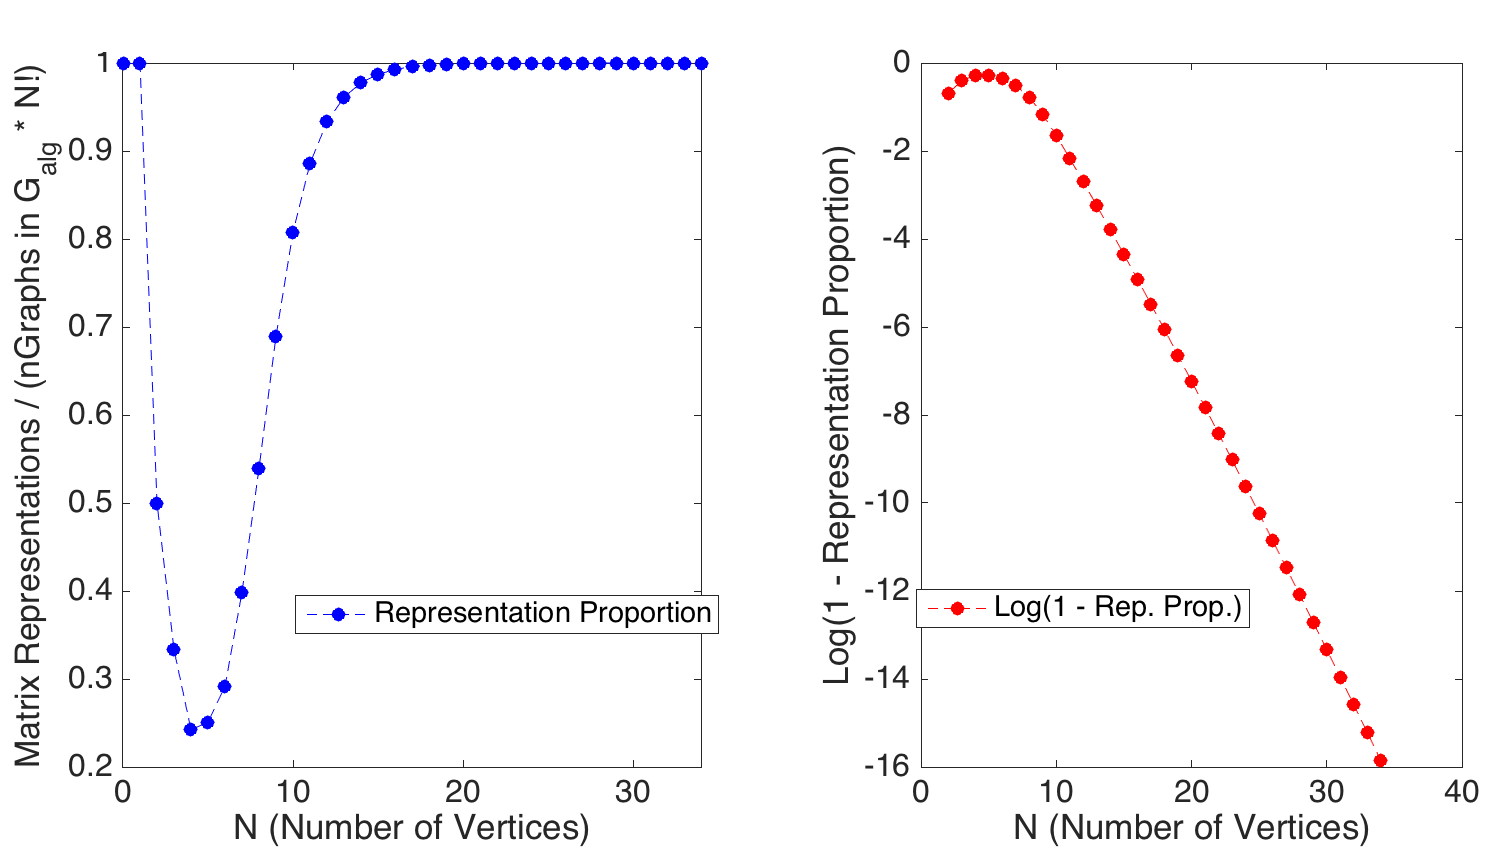
\includegraphics[width=\textwidth]{numGraphsAndMats}
\label{fig:mostgraphsoneaut}
\end{figure}

This should convince even a skeptical reader that for an average graph $g$ (even when treating it like an algebraic object), as $N$ increases, $\xoverline{|Aut(g)|} \rightarrow 1$.

\subsection{Implications for Perfectly Similar Vertex Sets}

Applying this back to our original purpose, we can surmise that the proportion of graphs which have only the trivial automorphism increases to one as $N$ increases.
In this common case, the SVSes are a set of $N$ distinct, one element sets, where each vertex is distinguishable from each other, and none share any automorphisms.
This makes checking for isomorphism between two random graphs trivial (if we have the SVSes), as the overwhelming majority of the time, we will only need to try the isomorphism implied by the direct, one to one mapping between the SVSes of the two graphs.

However, checking for automorphisms between every single pair of vertices is clearly in a higher computational complexity class than testing for isomorphism.
Thus, we will use smart heuristics to develop quazi-similar vertex sets, which will enable us to get the benefits of SVSes (i.e. implying the isomorphisms to try) without actually proving that the automorphisms that define the SVSes exist.

\section{Quazi-Similar Vertex Sets}

Quazi-Similar Vertex Sets (QSVSes) are constructed with respect to a vertex invariant, but have the same structure as SVSes.
The vertex invariant is calculated for all vertices within the graph, and those with the same value are placed into the same set.
Transitivity and reflexivity clearly both hold under this definition.
Moreover, the ordering/comparability of vertex invariants gives us a natural way to order the sets within the QSVSes.

In this section, we will describe how using the cycles invariant to generate QSVSes is highly successful at mirroring the true SVSes, and suggest an augmentation to cycles which correctly differentiates the two for a high proportion of cases.

\section{Why $P^*(G) <N$: Limitations on Cycles Usefulness}
\label{section:pstar}

\subsection{What is $P^*$, why does it matter?}

An ENORMOUS part of this thesis has thus far gone as assumed: what is $P$ (the maximum length cycle we are considering)?
When we are discussing cycles through a node, how long are the cycles we are considering?
The vertex invariant for cycles is clearly a vector, with the length of cycles corresponding to the place within the vector (cycles of length 2, 3, 4, etc.), but where do we draw the line?
To answer this question, I used a notion of `usefulness', to maximize the amount of information that we get out of the cycles invariant for the computation that we put into it.

Specifically, within the context of cycles as a vertex invariant, I started out with the assumption that all vertices share a single Similar Vertex Set (i.e. all are similar unless we have proof that they are not).
We then distinguish vertices by advancing P by one, we are in effect splitting this one class (or smaller classes) into even smaller classes, based on the information gleaned by increasing the length of all invariant vectors by one.
This kinds of `breaking-down' leads us to a concrete notion of usefulness: for a given graph G, cycles is useful at a power $P^*(G)$, where $P^*(G)$ is the minimum value for P at which all of the vertex sets in the SVSes are as broken down as they can get (for any larger values of P).
Thus, if we take the maximum of $P^*(G)$ across the set of all graphs over $N$ vertices and $M$ edges, , we will find a value $P^*(S_{N,M})$ at which point computation beyond this point is redundant for graphs over this set of graphs.
In this section we will be ignoring $M$, and examining the critical value for P over all values of $M$ while fixing $N$.
This would enable us to more concretely talk about running time, and its tradeoffs as a function of $N$ alone.
What we find (through both computational exploration and theoretical justification) is that $P^*(S_{N})$ can be described in direct terms of $N$:

\[ P^*(S_{N}) = \begin{cases} 
      N-1 & \text{If N is odd} \\
      N-2 & \text{If N is even} \\
   \end{cases}
\]

\subsection{Observational Data: Diameter vs. $P^*(G), G \in S_N$}

I first examined $P^*(G)$ as a function of the individual graph $G$, rather than over the set of all graphs, to try to see how the overall distribution of $P^*(G)$ looked for all graphs in the set.
Though this did not lead me anywhere directly, it did give me a clear idea of the upper bounds on $P^*(G)$ for an individual graph.
Shown in figure \ref{fig:diamvsmaxpower} is a description of this relationship.  By no means is it rigid, but the correlation is very strong between diameter and $P^*(G)$, labeled as $P_G$ on the y-axis.
It is also interesting (personally) just to see the diameter of a set of graphs laid out like this.

\begin{figure}[h]
\caption{\emph{Diameter Against $P^*(G)$ with $N=9$} - The size and number next to each circle tell us how many graphs (as algebraic objects) fit into different sizes of diameter and $P^*(G)$, labeled $P_G$}
\centering
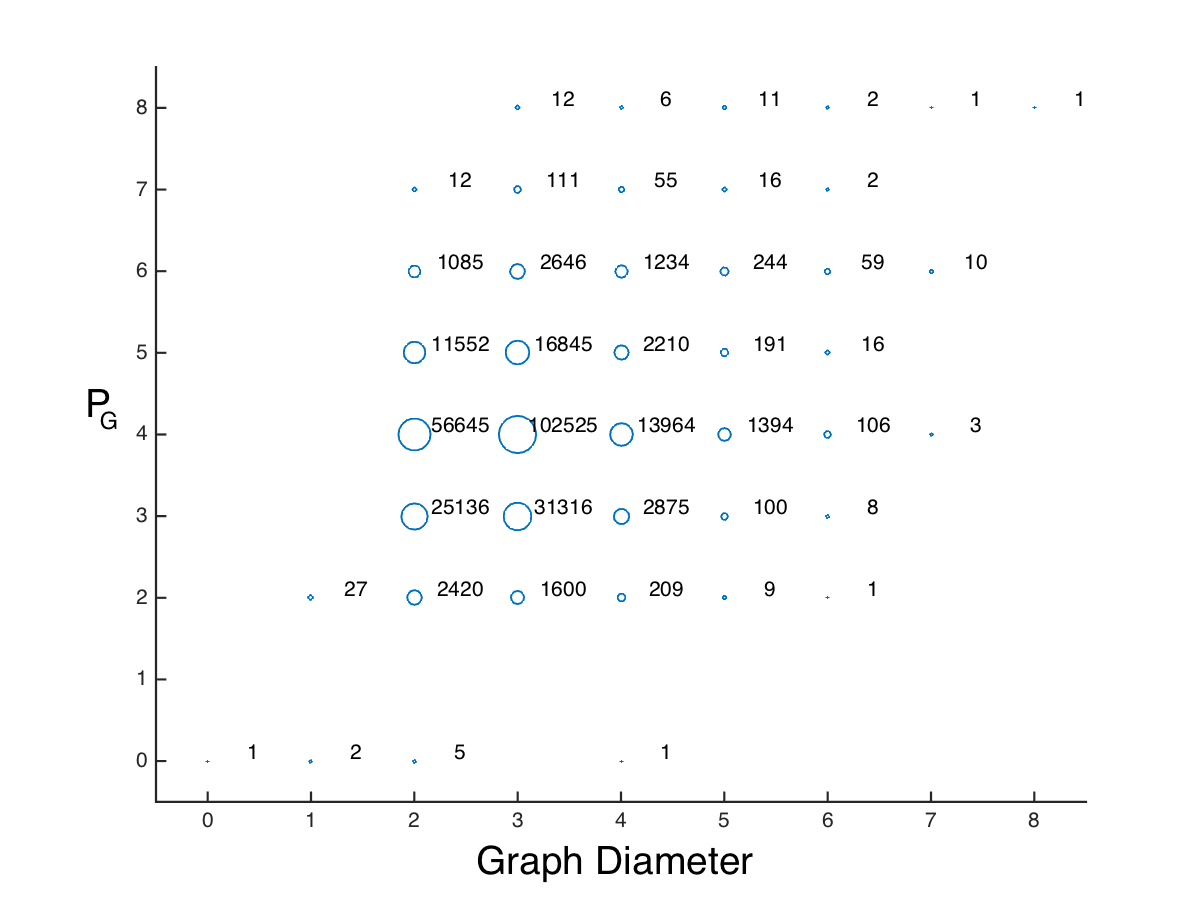
\includegraphics[width=\textwidth]{N9DiamVsDiffPower}
\label{fig:diamvsmaxpower}
\end{figure}

Four things are consistent across all of the alike graphs (shown in an appendix):
\begin{itemize}
\item{There is consistently a maximum diameter for $P^*(G)$, implying a $P^*(S_N)$ for each as shown in the table below}
\item{There are never any graphs with $P^*(G) = 1$, as we do not allow self loops }
\item{The Path graph ($P_N$), is always the lone member of the far upper right hand corner}
\item{The Cycle graph ($C_N$), always has $P^*(G)$ equal to that of the Path graph: $P^*(C_N) = P^*(P_N)$}
\end{itemize}
The upper bound proposed by each one of the values for $P^*(S_N)$ follows the pattern:
\[ P^*(S_N) = \begin{cases} 
      N-1 & \text{If N is odd} \\
      N-2 & \text{If N is even} \\
   \end{cases}
\]
for $N <=9$. This sets up a strong case for this as a target hypothesis, but we still must prove it.

\subsection{Theoretical Justification: $P_N$ versus $C_N$}
Why does the proposed value for $P^*(S_N)$ make sense?

This proof consists of two parts, the first is why $P^*(P_N) = \text{the proposed} P^*(S_N)$ for the Path graph ($P_N$), the second describes why all other graphs $G$ have $P^*(G) \leq P^*(P_N)$.

Part 1: \emph{Distinguishing between vertices in the path graph requires $P^*(P_N) = N - 1 - ((N+1)\%2)$.}

Start all vertices in the same assumed similarity set, and assume that $P = 0$.
When we increase $P$ to 2, all vertices have degree 2 (the second entry in the cycles invariant) except for the two terminuses, thus the two terminuses are split off from the original quazi-similarity set, as they have been distinguished at $P=2$ by their cycles invariant.
When we increase $P$ to 4, the two nodes adjacent to the two terminuses are now distinguished (as they are now `missing' a path of length four that they would have had if they were further in toward the center of the path graph). 
There are now $N-4$ vertices remaining in the original quazi-similar vertex set.
From this, it is clear to see that for an arbitrarily large path graph, for $P=2K$, there will be $N-2K$ elements in the original QSVS.
We will have \emph{fully distinguished} all of the vertices into distinct QSVSes which are true to the SVSes when the original QSVS contains only the `middle' node(s).

In the even case $N = 2K, K \in Z$, this occurs when we have 
$$P^*(P_N) = 2\ceil{\frac{N-2}{2}} = 2\ceil{\frac{2K}{2} - 1} = 2\ceil{K - 1} = 2(K - 1) = 2K - 2 = N - 2$$
In the odd case $N = 2K +1, K \in Z$, this occurs when we have 
$$P^*(P_N) = 2\ceil{\frac{N-2}{2}}  = 2\ceil{\frac{2K+1- 2}{2}} = 2\ceil{K - 1/2} = 2K = N - 1 $$

Thus, we know that 
\[ P^*(P_N) = \begin{cases} 
      N-1 & \text{If N is odd} \\
      N-2 & \text{If N is even} \\
   \end{cases}
\]

Part 2: \emph{Why is $\forall g \,\in\, S_{N} , \;P^*(P_N) \geq P^*(g)$? Why is the path the hardest to internally distinguish?}

Cycles invariant calculation is a form of vertex coloring for isomorphism testing, with the feature that distinguishes vertices being the number of cycles that pass through them of given lengths.
Since $P^*$ is concerned with the largest value of Cycles able to all nodes from one another internally, we know that the graph that is the hardest to internally distinguish will (1) at least have two distinct groups (if not more) of vertices within it, and (2) will have a slow traversal of its colorings (which is a function of its girth, the maximum distance between two nodes in the graph).
If we can distinguish any pair of vertices from one another at any level (if at the degree sequence, at P=2, or at the number of triangles, P=3, etc.), then we can distinguish the vertices which are only attached to one of the pair members that we distinguished at $P+2$, as that new cycle will be reverberated to the connected vertices with cycles that can traverse to the distinguished node, complete the cycle, and return back.
Thus, cycles, propagates in such a way that whenever we can make a single distinction of two nodes (say $v_j$ and $v_k$) in the graph (lets say at $P=p_0$), then all nodes in the graph will be as distinguished as they are able to be via Cycles at $P=K+2*max\big[min\big(dist(v_i,v_j), dist(v_i,v_k)\big)\big]$.
It is clear that the maximum value of the maximum term is half the value of the girth of the graph (as in the worst case, $v_j$ and $v_k$ are the vertices that are furthest apart, defining the girth, and the distance between $v_i$ and one of the two vertices is maximized when $v_i$ is equidistant from each. 
Thus, we can change this expression into $P=K+girth(G)$.
Meaning there are two different ways to try to maximize this expression with respect to P (as that is what we are really trying to find), we could either try to maximize it by maximizing the girth or by maximizing K.
Since K is a function of the first feature that can be distinguished, it is clear that $K$ will be strictly less than $N$ (as if we get to that point, then we will not be able to make any distinctions).
Thus, the way to maximize $P$ is to maximize the girth.
This occurs in the path graph ($P_N$).
Thus no graph can have larger $P^*(G)$ than the path graph.

The combination of these two claims proves that the expression 
\[ P^*(G) \leq \begin{cases} 
      N-1 & \text{If N is odd} \\
      N-2 & \text{If N is even} \\
   \end{cases}
\]
holds for all graphs, a useful piece of knowledge in curtailing the amount of computational work we must do. 

\section{Improving upon QSVS with Flagged Cycles}

The quality of the QSVS is generally described as how close they are to the true SVSes.
In other words, quality is a measure of how frequently does a QSVS contain two or more subsets that should be independent SVSes.
Though Cycles as a vertex invariant produces QSVSes which mirror SVSes with high probability, we should examine the failures cases to see if we can do better.

We will accomplish this via a methodology I am calling `flagging' after I have seen that a few times in the literature.
Flagging (or Marking) is the process of taking a graph and appending a single vertex to it which is connected by a single edge to some target vertex in the graph.
Flagging frequently modifies graph structure enough to see impacts which successfully differentiate between non-isomorphic/non-automorphic structures.

For example, if we have two co-spectral graphs, and we are curious whether or not an isomorphism exists between the two of them, we can append a flag on each one of the vertices which must be mapped together in a potential isomorphism, and then take the chromatic polynomial again.
If the new (flagged) graphs differ in their chromatic polynomial, then the two vertices that were flagged cannot have an isomorphism to one another, as modifying two isomorphic graphs in a systematically consistent way should preserve isomorphism.
We use this principle in the pursuit of fully differentiating a set of QSVS into a refined state that is more likely to equal the ground-truth SVSes.

\subsection{Appending a Flag, Somewhat Predictable}

Our methodology for modifying the QSVSes is simple: first, calculate the QSVSes using the Cycles invariant.
For each of the sets within the QSVSes with more than one element, perform a flagging operation K times, if the set has K elements, which results in K different graphs.
Calculate the cycles graph invariant over each of these graphs.
If the cycles invariants for any two of the K graphs differs, then split apart the set of vertices into two (or more) new QSVSes, one for each different value of the graph invariant associated with the graph formed by flagging each vertex.

An interesting piece of this is that we can actually predict some of the values that the newly created, flagged graphs, will have for their cycles invariant values.
Specifically, if we are given the previous value of the cycles invariant, and told which vertex in the cycles invariant is going to be appended to, we can predict the number of cycles for the flag vertex (the new vertex), as each one of the cycles that it is a part of must go to and from the flagged vertex (the vertex the new vertex was attached to), and we already knew how many of those there were from the original cycles function.
Additionally, we can predict the change in the number of cycles for the flagged vertex, as we knew its cycle profile before, and the addition of a single vertex on to it can be interpreted as a recursive definition, where cycles are broken into components that travel back (and forth) from the flag vertex and those that exist within the graph.
Though difficult to explain via formulae and words, I would encourage a skeptical reader to check out my code at (/Thesis/Matlab/constituentpaths/predictPathsOfAddingOneVertex.m).

Equally interesting (to the fact that we \emph{can} predict Cycles for these two nodes when just given the Cycles invariant) is that we \emph{cannot} make any further predictions about the flagged cycles values based solely on the plain cycles values.
We know this to be true because in Co-Cycles graphs, we frequently get different flagged cycles graph invariants when we flag vertices which are suggested to be isomorphic (but are not).
This is a good piece of information to know because it gives us proof that flagging is not some kind of manipulation of information that we already have, it represents a way to get pieces of information that include additional structural information.

\subsection{Intuitive Justification for Flagging}

This section is not grounded in proof, but gives a conceptual reason that flagging works at further discriminating between vertices that we think might be automorphic.
Cycles is really a rough description of the `neighborhood' of a vertex within its context in the graph.
Cycles tells us about the way that the structure reverberates, it is, in many ways, a description of resonance.
One conceptual tool I like is to think about electricity flowing (bidirectionally) around a circuit, and measuring the self-connectivity or resistance between points based on the number of ways that electrons could flow.

Flagging a node changes that resonance.
It changes it in a way that we understand and can predict for the flagged vertex and the flag vertex.
However, it also changes the way that cycles `reverberate' through the flagged vertex, and in doing so, changes the cycles invariant at other vertices.
We can even think of this in more concrete terms: take the cycles invariant for the flagged graph (without sorting), then subtract off the cycles invariant for the non-flagged graph (again, without sorting).

This tells you exactly how many new cycles have been created which pass through the flagged node at least once.
We call this modified matrix the \emph{excess cycles} matrix.
Note that this is \emph{not} the same as the row for the flagged cycles matrix, and actually encodes significantly more information (the constituents of those cycles, not only that they exist).
In doing so, we actually get tangible information about the connectivity of each of the nodes.
From the excess cycles matrix, we can calculate the distance between the flagged vertex and each of the other vertices in the graph.
We can calculate the relative makeup of each of the added cycles (how many pass through each vertex, and how many times does each double back on itself), among a large number of other features.

The intuitive justification for flagging is compelling, and if I had another month to puzzle away at this problem, this is probably the area I would spend the most time focusing on.

\subsection{Analytical Support: Strength of Cycles as Vertex Invariant}

The analytical support for flagging is strong:
for all graphs of size $N < 10$, cycles with flagging as a mechanism for QSVS generation correctly generated QSVSes which perfectly estimated (without flaws) the accurate SVSes.
Few examples were found for $N \geq 10$, though some were.

To give the reader an idea of how useful Cycles (and flagged Cycles) are at discriminating between vertices in graphs, I performed some random trials to attempt to estimate their failure rate.
By failure here, I mean the probability that the QSVSes generated by the invariant are \emph{not} equal to the SVSes that can be found via brute force/automorphism examinations.
Note that this kind of failure is only a lack of perfect distinction, it never means a false negatives, in similar vertex testing false negatives are impossible by either methodology.

In figure \ref{fig:proportionQSVSeqSVS}, you can see the results of a trial which generated 1,000,000 random graphs of size 10, 11 and 12, and calculated the proportion of each that are fully distinguished into their correct Similar Vertex Sets by each methodology of generating them.
What we find is that it appears that as the number of vertices increases, the overall number of graphs which fails this metric decreases, a valuable result.
Additionally, we see that the overall number which fail is very low, which is heartening, and gives us good reason to believe that these are both high quality vertex invariants.

\begin{figure}[h]
\caption{\emph{Proportion of all graphs where SVSes = QSVSes generated by two Methodologies}}
\centering
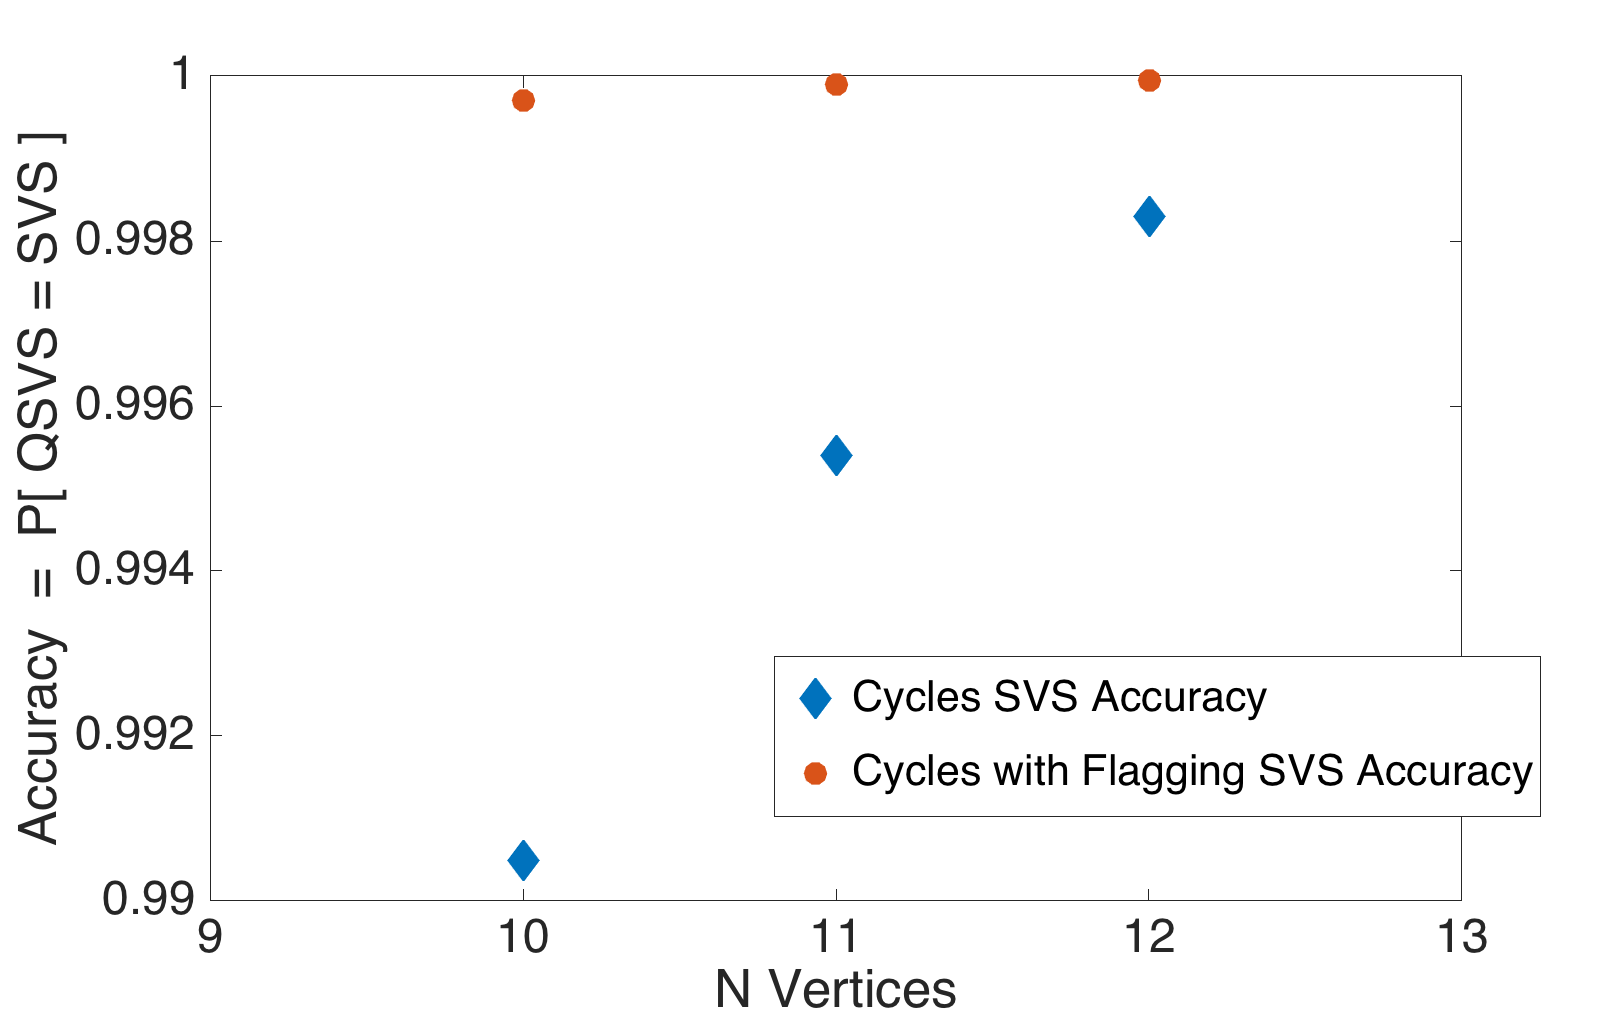
\includegraphics[width=\textwidth]{proportionExploredv10to12}
\label{fig:proportionQSVSeqSVS}
\end{figure}



